\setchapterimage[3.5cm]{mma/crab-page}
\setchapterpreamble[u]{\margintoc}
\chapter{Summary and Future Outlook}
\labch{summary}
\begin{fquote}[Ambrose Bierce][The Cynic's Dictionary][1906] FUTURE, n. That period of time in which our affairs prosper, our friends are true and our happiness is assured.  
\end{fquote}

LSST

Ligo O4 + LIGO India + Kagra -> Many kilonovae -> Hubble constant, test general relativity, 

IceCube Gen2 + PeV band + KM3net + Baikal + P-One

Radio


\begin{marginfigure}
	\centering 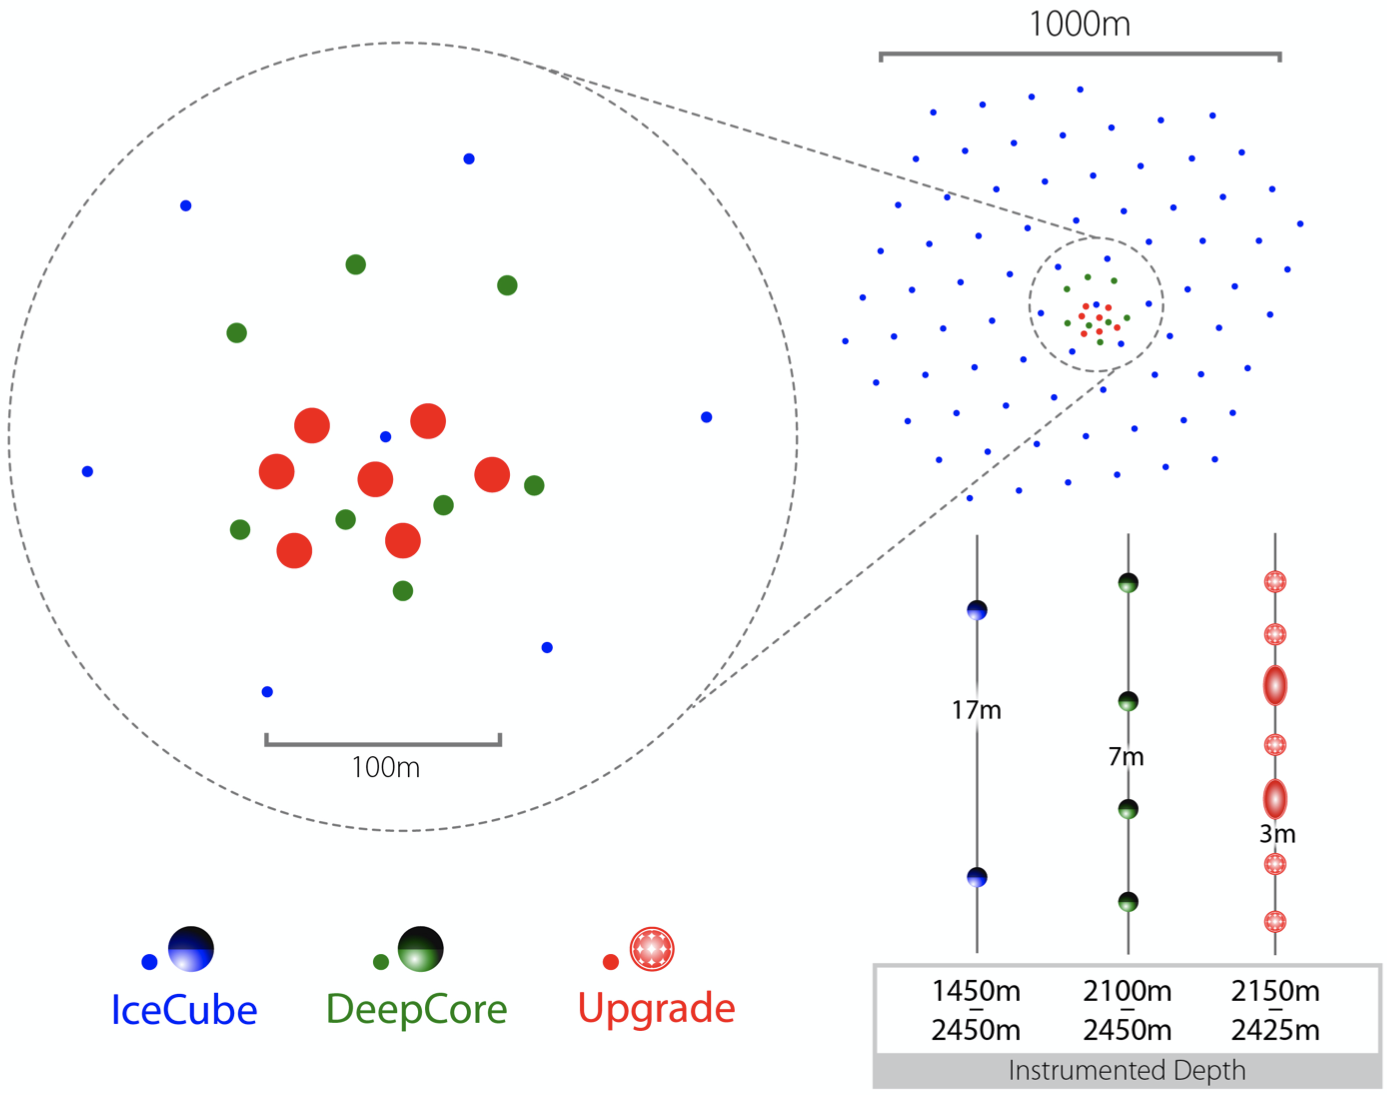
\includegraphics{outlook/icecube_upgrade}
	\caption{Layout of the IceCube Upgrade, with figure from \cite{ic_upgrade}.}
	\label{fig:upgrade}
\end{marginfigure}

In the near future, the seven-string \emph{IceCube Upgrade} will be deployed. This dense in-fill array is primarily designed to extend IceCube's sensitivity to lower-energy (GeV) neutrinos, and will thus most directly impact studies of neutrino oscillations and low-energy transients. However, the IceCube Upgrade also includes extensive calibration hardware, and may thus have a large indirect impact on IceCube neutrino astronomy performance. Better modelling of uncertainties such as the ice properties may lead to substantially-revised reconstructions and angular error estimates, and thus reveal previously-obscured correlations in archival neutrino data.

\begin{marginfigure}
	\centering 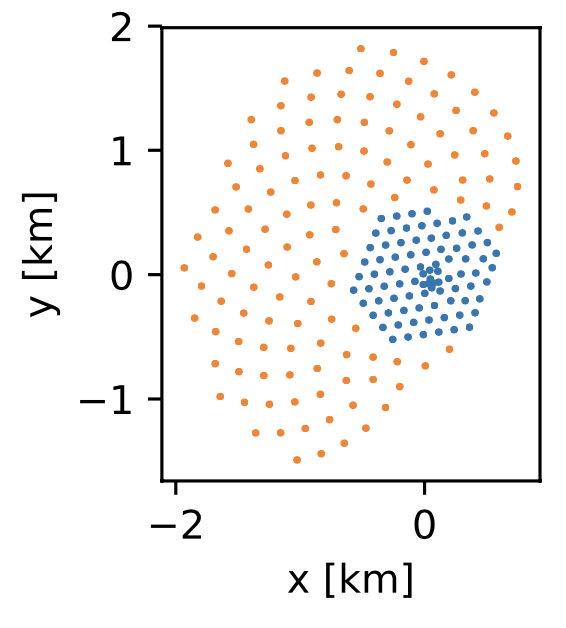
\includegraphics{outlook/gen2_layout}
	\caption{Layout of IceCube-Gen2 in comparison to IceCube, from \cite{gen2_icrc}.}
	\label{fig:gen2_layout}
\end{marginfigure}

However, more significantly, the \emph{IceCube-Gen2} extension should begin deployment this decade \cite{gen2_icrc}. This would expand the instrumented volume from the current 1 km$^{3}$ to a total of 7.9 km$^{3}$. To be cost-effective, the new volume would have a lower DOM density. Thus, though the rate of high-energy neutrino detections will substantially increase, the reduction DOMs will impact event reconstruction, particularly at lower energies. While the individual DOMs themselves are likely to be more effective, IceCube-Gen2 will still represents a transition in energy range, with a median energy of 30 TeV rather than  10 TeV for IceCube. This transition is also relevant in terms of sensitivity, because the IceCube detector has operated primarily as a 4$\pi$ detector, or at least a $2 \pi$ one. However, for higher energies the impact of Earth absorption becomes more significant, so as seem in Figure \ref{fig:gen2_sens} the enhanced sensitivity of the detector at the horizon will become somewhat more pronounced.  Radio will...

\begin{marginfigure}
	\centering 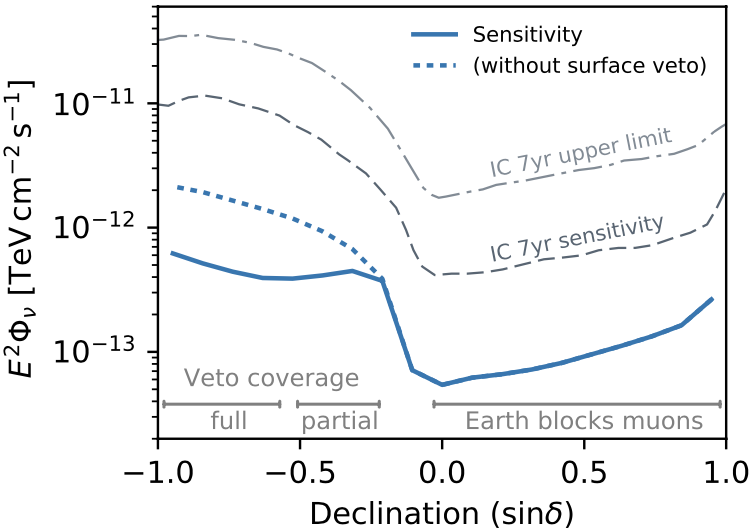
\includegraphics{outlook/gen2_sens}
	\caption{Sensitivity of IceCube-Gen2 (orange) in comparison to IceCube (blue), from \cite{gen2_icrc}. The dotted line shows the sensitivity without surface veto.} 
	\label{fig:gen2_sens}
\end{marginfigure}

The AMANDA detector discovered atmospheric neutrinos, and served as a stepping stone to IceCube. IceCube, now in full operation for over a decade, successfully established neutrino astronomy with the discovery of he astrophysical neutrino flux, but has a characteristic signal-to-noise which has so far only proved sufficient to provide 3$\sigma$ hints of neutrino sources. With luck, IceCube-Gen2 could mark the transition of neutrino astronomy to a mature field, in which 5$\sigma$ discoveries become routine. At this point, focus will shift from finding sources to characterising them. Neutrino population studies, indeed neutrino tomography and spectroscopy, are powerful scientific tools that we are not yet capable of leveraging, but could in future teach us much about astrophysical objects. Further, a well-characterised flux of astrophysical neutrinos would also provide an ideal tool for testing particle physics at the very highest energies.

Gen2 sensitivity plot?

Ultrasat -> UV photon science

CTA

eROSITA

Automation + ML -> Probabilistic classification for stacking
Realtime all the time

More TDEs, new stacking analysis